\documentclass[
11pt, % Set the default font size, options include: 8pt, 9pt, 10pt, 11pt, 12pt, 14pt, 17pt, 20pt
%
aspectratio=169, % Uncomment to set the aspect ratio to a 16:9 ratio which matches the aspect ratio of 1080p and 4K screens and projectors
]{beamer}

\graphicspath{{Images/}{./}} % Specifies where to look for included images (trailing slash required)
\usepackage{booktabs} % Allows the use of \toprule, \midrule and \bottomrule for better rules in tables
%\usepackage{enumitem}
%\usepackage{appendixnumberbeamer} %If you want a separate slide counter for your appendix

%%% Customize Theme %%%%%%%%%%%%%%%%%%%%%%
\usetheme{Madrid} % You can use other themes too, but this changes many things. I've found Madrid to be the best for this color scheme

%fg = font color
%bg = background color

% ! WARNING ! : Many colors are linked to multiple attributes, so changing one color can have unexpected changes!

% If you want to tweak the shading of orange and red, tweak the below 2 lines:t
\definecolor{myGreen}{RGB}{0,155,125}
\definecolor{myDarkGreen}{RGB}{1, 93, 82}

% Bottom right hand color
\setbeamercolor*{structure}{bg=myGreen!20,fg=myGreen!90}

\setbeamercolor*{palette primary}{use=structure,fg=white,bg=structure.fg} %?
\setbeamercolor*{palette secondary}{use=structure,fg=myGreen,bg=white}
%bottom left of footer & bar between title & top bubbles
\setbeamercolor*{palette tertiary}{use=structure,fg=white,bg=myGreen} 

\setbeamercolor{frametitle}{bg=myGreen!85,fg=white} %title of each slide

\setbeamercolor*{titlelike}{parent=palette primary} %?
%\setbeamercolor{titlelike}{parent=palette primary,fg=structure.fg!50!myRed}

%for miniframe (very top) AND center footer
\setbeamercolor{section in head/foot}{fg=myDarkGreen, bg=white}

%%% Specific Colors %%%
\setbeamercolor{item projected}{bg=myDarkGreen}
\setbeamertemplate{enumerate items}{bg=myOrange}

\setbeamercolor{itemize item}{fg=myDarkGreen}
\setbeamercolor{itemize subitem}{fg=myDarkGreen}

\setbeamercolor{button}{bg=myDarkGreen}

%%% Edits ONLY the TOC slide %%%
\setbeamercolor{section in toc}{fg=black}
\setbeamercolor{subsection in toc}{fg=black}

%%% Block Colors %%%
% Standard block %
\setbeamercolor{block title}{bg=myDarkGreen, fg=white}
\setbeamercolor{block body}{bg=myDarkGreen!20}

% Alerted block % If you want to customize it's color
%\setbeamercolor{block title alerted}{bg=cyan, fg=white}
%\setbeamercolor{block body alerted}{bg=cyan!10}

% Example block % If you want to customize it's color
%\setbeamercolor{block title example}{bg=cyan, fg=white}
%\setbeamercolor{block body example}{bg=cyan!10}

%---------------------------------------------------------
%	SELECT FONT THEME & FONTS
%---------------------------------------------------------
\usefonttheme{default} % Typeset using the default sans serif font
\usepackage{palatino} % Use the Palatino font for serif text
\usepackage[default]{opensans} % Use the Open Sans font for sans serif text
\useinnertheme{circles}

%---------------------------------------------------------
%	SELECT OUTER THEME
%---------------------------------------------------------
% Outer themes change the overall layout of slides, such as: header and footer lines, sidebars and slide titles. Uncomment each theme in turn to see what changes it makes to your presentation.

%\useoutertheme{default}
%
\useoutertheme{miniframes}

%\useoutertheme{infolines}
%\useoutertheme{smoothbars}
%\useoutertheme{sidebar}
%\useoutertheme{split}
%\useoutertheme{shadow}
%\useoutertheme{tree}
%\useoutertheme{smoothtree}

%---------------------------------------------------------
%	PRESENTATION INFORMATION
%---------------------------------------------------------

\title[Descubrimiento de Conocimiento M\'edico]{Descubrimiento de Conocimiento M\'edico}
\subtitle{Proyecto de Aprendizaje de M\'aquinas}
\author[]{Diamis Alfonso \\ Mari\'e del Valle \\ Roxana Pe\~na \\ Dennis Fiallo \\ Ernesto Alfonso \\ Rolando Sanch\'ez}

\date{}

%\date[\today]



%---------------------------------------------------------
%---------------------------------------------------------
%---------------------------------------------------------
\begin{document}
	
	%---------------------------------------------------------
	%	TITLE SLIDE
	%---------------------------------------------------------
	\section{}
	\begin{frame}
		\titlepage % Output the title slide, automatically created using the text entered in the PRESENTATION INFORMATION block above
		
	\end{frame}
	
	%---------------------------------------------------------
	%	TABLE OF CONTENTS SLIDE
	%---------------------------------------------------------
	% The table of contents outputs the sections and subsections that appear in your presentation, specified with the standard \section and \subsection commands. You may either display all sections and subsections on one slide with \tableofcontents, or display each section at a time on subsequent slides with \tableofcontents[pausesections]. The latter is useful if you want to step through each section and mention what you will discuss.
	
	%\begin{frame}
	%	\frametitle{Table of Contents} % Slide title, remove this command for no title
	%	
	%	\tableofcontents % Output the table of contents (all sections on one slide)
	%	%\tableofcontents[pausesections] % Output the table of contents (break sections up across separate slides)
	%\end{frame}
	
	%---------------------------------------------------------
	%	PRESENTATION BODY SLIDES
	%---------------------------------------------------------
	\section{Objetivo} % Sections are added in order to Organize your presentation into discrete blocks, all sections and subsections are automatically output to the table of contents as an overview of the talk but NOT output in the presentation as separate slides
	
	%------------------------------------------------
	\begin{frame}
		\frametitle{Objetivos del proyecto}
		\begin{itemize}
			\item Utilizar técnicas de machine learning y procesamiento del lenguaje natural para descubrir y extraer conocimiento médico a partir de la data de ehealthkd2021.
			
			
		\end{itemize}
	 	
	
	
	\end{frame}

     \section{Data}
      %------------------------------------------------
     \begin{frame}
     	\frametitle{Data}
     	\begin{itemize}
     		\item Los datos son oraciones en español e inglés presentes en la data de ehealthkd2021. Esta base de datos contiene información médica relevante, como informes de pacientes, notas clínicas y registros médicos, en ambos idiomas.
     		
     	\end{itemize}
     
     	
     \end{frame}
     
     %------------------------------------------------
     %------------------------------------------------
     \section{Tareas}
     
     \begin{frame}
     	\frametitle{Tareas}
     	Entre las tareas a implementar se encuentran:
     	\begin{enumerate}
     		\item[1.] \textbf{ Named Entity Recognition (NER)}: \\
     		
     		Identificar y clasificar entidades en el texto. Se cuentan con 4 tipos de entidades.
     		\begin{itemize}
     			\item Concept
     			\item Action
     			\item Predicate
     			\item Reference
     		\end{itemize}
     		
     	\end{enumerate}
     	
     	
     \end{frame}
 
 	  \begin{frame}
 		\frametitle{Tareas}
 		
 		\begin{enumerate}			
  			\item[2.] \textbf{Relation Extraction (RE)}:\\
  			
  			 Identificar las relaciones y las conexiones entre las entidades en el texto. Se tienen las relaciones siguientes.
  			 \begin{itemize}
  			 	\item is-a
  			 	\item same-as
  			 	\item has-property
  			 	\item causes
  			 	\item entails
  			 	\item in-time
  			 	\item subject
  			 	\item target
  			 	\item domain
  			 	\item arg
  			 	
  			 \end{itemize}
  			 
 			\item[3.] \textbf{Combinación de NER y RE}.
 		\end{enumerate}
 		
 		
 	\end{frame}
	
	%------------------------------------------------
	%------------------------------------------------
	\section{Modelos}
	
	\begin{frame}
		\frametitle{LSTM (Long Short-Term Memory)}
		\begin{block}{Definici\'on}
			Es un tipo de red neuronal recurrente (RNN) que se utiliza para procesar y analizar secuencias de datos, como texto, audio o series de tiempo. A diferencia de las RNN tradicionales, que pueden tener dificultades para capturar relaciones a largo plazo en los datos, las LSTM están diseñadas específicamente para resolver este problema mediante el uso de celdas de memoria.
		\end{block}
	
		
	%	\begin{figure}[h!]
	%		\centering
	%		%\caption{}
	%		\includegraphics[scale=0.5]{../Imagenes/campos receptivos sin campo visual}
	% 		%\label{fig}
	%	\end{figure} 	
		
		
	\end{frame}
	
	%------------------------------------------------
	%------------------------------------------------
	\begin{frame}
		\frametitle{BERT (Bidirectional Encoder Representations from Transformers)}
		
		\begin{block}{Definici\'on}
			Es un modelo de lenguaje basado en la arquitectura Transformer desarrollado por Google. A diferencia de los modelos de lenguaje tradicionales, que se entrenan de manera unidireccional, BERT se entrena de manera bidireccional, lo que le permite capturar el contexto de las palabras en una oración de manera más efectiva.
		\end{block}
		
	%	\begin{figure}[h!]
	%		\centering
	%		%\caption{}
	%		\includegraphics[scale=0.4]{../Informe/JCE Estudio_de_la_proyección_de_estímulos_visuales_a_la_corteza_visual/Images/campo receptivo-2}
	%		%\label{fig}
	%	\end{figure} 	
	%	
		
	\end{frame}
	
	%------------------------------------------------
	
	%------------------------------------------------
	\begin{frame}
		\frametitle{T5 (Text-To-Text Transfer Transformer))}
		\begin{block}{Definici\'on}
			Es un modelo de lenguaje basado en la arquitectura Transformer y diseñado específicamente para la transferencia de texto a texto, lo que significa que puede abordar una amplia gama de tareas de procesamiento del lenguaje natural (NLP) mediante la formulación de la entrada y la salida en un formato de texto a texto.
		\end{block}
	
	\end{frame}
	%------------------------------------------------
		%------------------------------------------------
	\begin{frame}
		\frametitle{GPT-3 (Generative Pre-trained Transformer 3)}
		
		\begin{block}{Definici\'on}
			Es un modelo de lenguaje desarrollado por OpenAI. Es la tercera versión de la serie GPT y se basa en la arquitectura Transformer. Puede generar texto coherente y contextualmente relevante en respuesta a una entrada de texto.
		\end{block}
		
	%	\begin{figure}[h!]
	%		\centering
	%		%\caption{}
	%		\includegraphics[scale=0.5]{../Informe/JCE Estudio_de_la_proyección_de_estímulos_visuales_a_la_corteza_visual/Images/monopolo y dipolo}
	%		%\label{fig}
	%	\end{figure} 	
		
	\end{frame}
	%------------------------------------------------
	\section{Resultados}
	%------------------------------------------------
	\begin{frame}
		\frametitle{NER}
		
				\begin{figure}[h!]
					\centering
					%\caption{}
					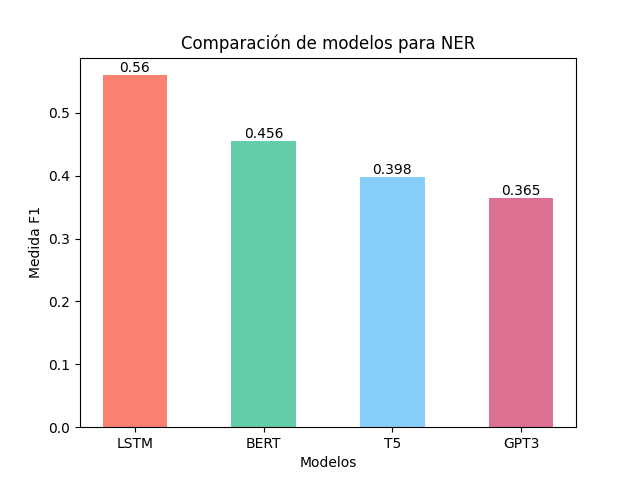
\includegraphics[scale=0.5]{../images/NER_bar}
					%\label{fig}
				\end{figure} 	
		
	
		
	\end{frame}
	
	%------------------------------------------------
	\begin{frame}
		\frametitle{RE}
			\begin{figure}[h!]
			\centering
			%\caption{}
			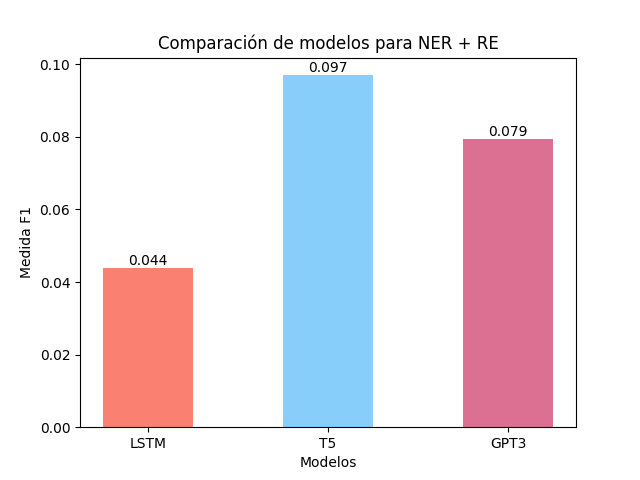
\includegraphics[scale=0.5]{../images/RE_bar}
			%\label{fig}
		\end{figure} 	
		
		
	\end{frame}
	
	%------------------------------------------------
	%------------------------------------------------
	\begin{frame}
		\frametitle{Combinaci\'on NER y RE}
				
		\begin{figure}[h!]
		\centering
		%\caption{}
		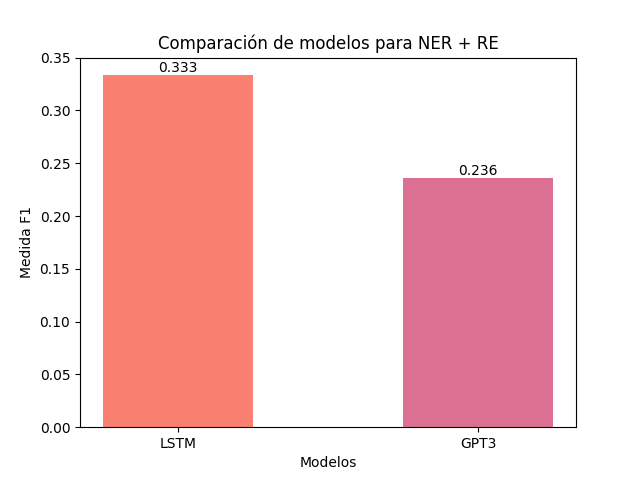
\includegraphics[scale=0.5]{../images/NER_RE_bar}
		%\label{fig}
	\end{figure} 	
			
		
	\end{frame}
	
	%------------------------------------------------
	\section{Ontolog\'ias}
		%------------------------------------------------
	\begin{frame}
		\frametitle{Ontolog\'ias}
		
		Una vez obtenido todo el conocimiento de los documentos, se guardan los datos en una base de datos orientada a grafos. 	
		Para ello se utiliza \textbf{Neo4j}, el cual permite acceder a los datos de diversas formas y usando distintos lenguajes de consulta. En nuestro proyecto se utiliza \textbf{Cypher}, un lenguaje que permite consultar y manipular grafos.
		
	\end{frame}
	
	\begin{frame}
		\frametitle{Ontolog\'ias}
		
		La comunicación con la base de datos se realiza en el siguiente método:
		
			\begin{figure}[h!]
			\centering
			%\caption{}
			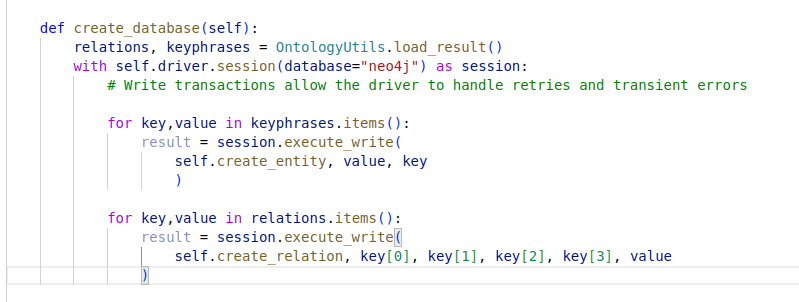
\includegraphics[scale=0.5]{../images/createdatabase.png}
			%\label{fig}
		\end{figure} 	
		
		
	\end{frame}

	\begin{frame}
		\frametitle{Ontolog\'ias}
		
		La generación de los nodos como entidades la realizamos con las siguientes consulta:
		
		\begin{figure}[h!]
			\centering
			%\caption{}
			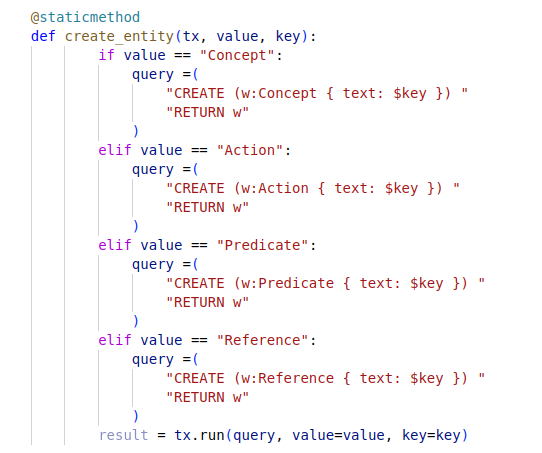
\includegraphics[scale=0.3]{../images/imageEntities.png}
			%\label{fig}
		\end{figure} 	
		
		
	\end{frame}

	\begin{frame}
		\frametitle{Ontolog\'ias}
	
		Para la creación de las relaciones entre los nodos utilizamos la consulta:
		
		\begin{figure}[h!]
			\centering
			%\caption{}
			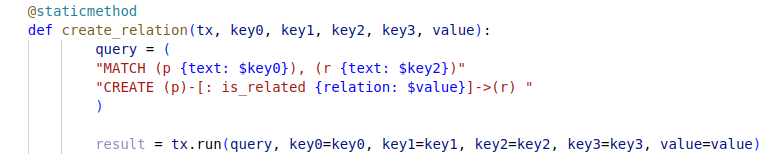
\includegraphics[scale=0.5]{../images/imageRelations.png}
			%\label{fig}
		\end{figure} 	
	\end{frame}
	
	\begin{frame}
		\frametitle{Ontolog\'ias}
		
		Este método realiza una consulta para conocer las causas de alguna enfermedad de interés:
		
		\begin{figure}[h!]
			\centering
			%\caption{}
			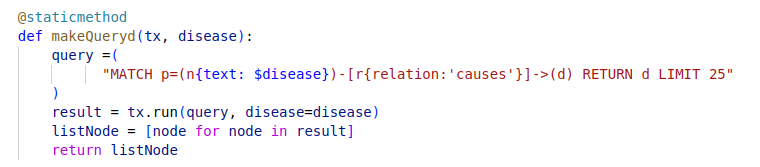
\includegraphics[scale=0.5]{../images/imageQuery.png}
			%\label{fig}
		\end{figure} 	
	
	
	\end{frame}

		\begin{frame}
		\frametitle{Ontolog\'ias}
		
		En esta imagen podemos ver los resultado obtenidos al realizar la consulta para conocer las causas del covid-19:
		
		\begin{figure}[h!]
			\centering
			%\caption{}
			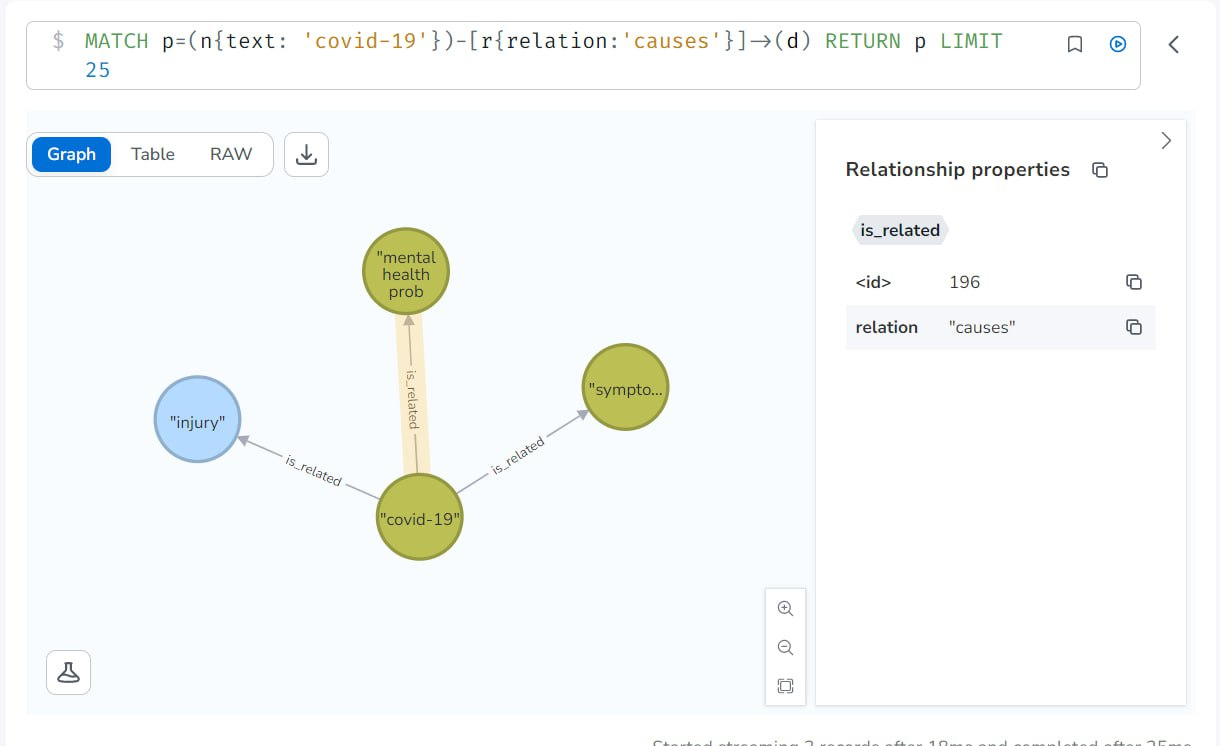
\includegraphics[scale=0.3]{../images/imagecons.png}
			%\label{fig}
		\end{figure} 	
		
		
	\end{frame}

	\begin{frame}
	\frametitle{Ontolog\'ias}
	
		\begin{figure}[h!]
		\centering
		%\caption{}
		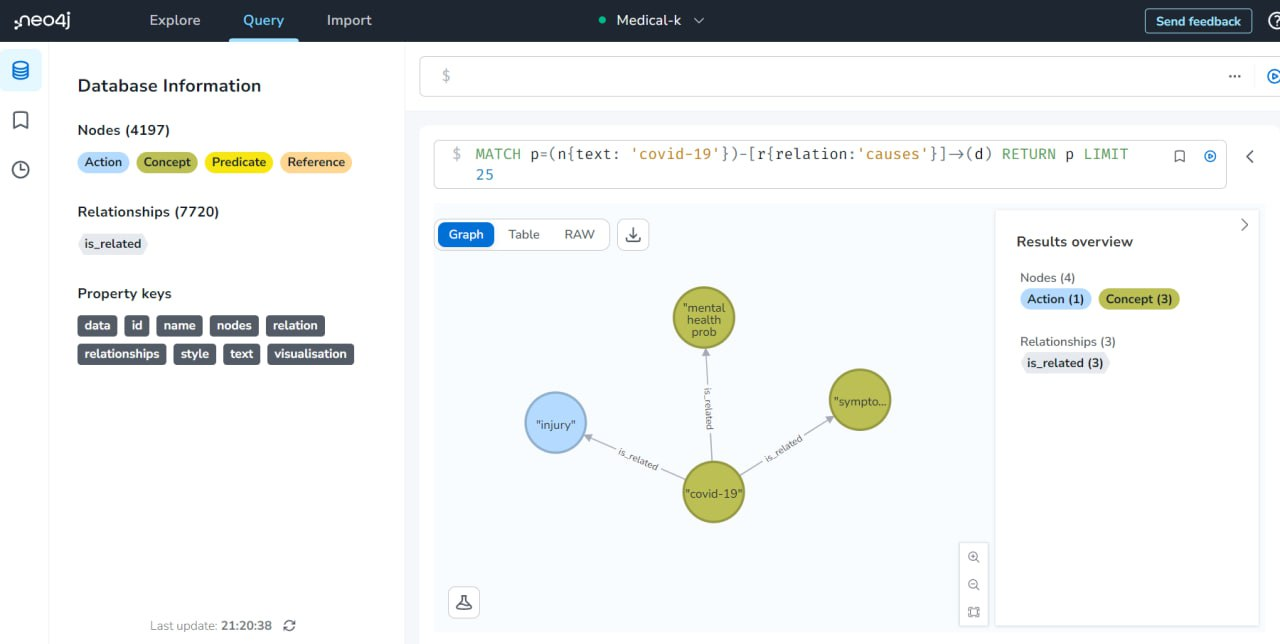
\includegraphics[scale=0.3]{../images/imagecons1.png}
		
		%\label{fig}
		
	\end{figure} 	
	
	
	\end{frame}

		\begin{frame}
		\frametitle{Ontolog\'ias}
		
		\begin{figure}[h!]
			\centering
			%\caption{}
		
			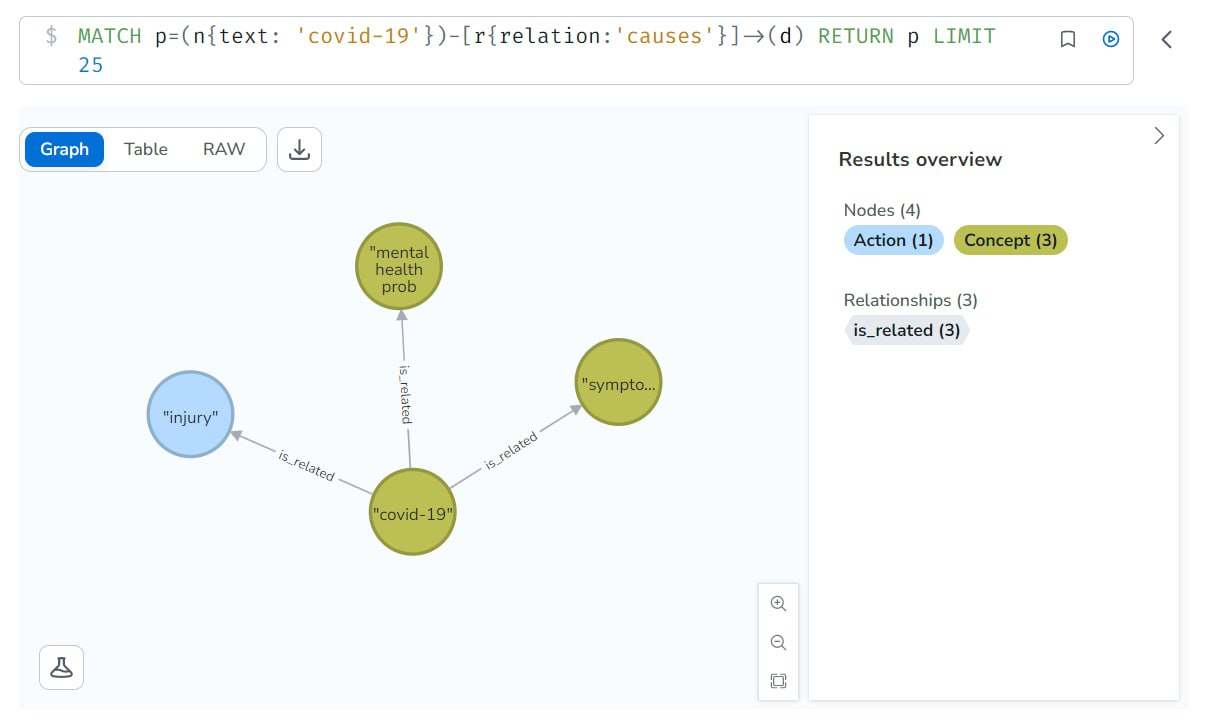
\includegraphics[scale=0.3]{../images/imageconsulta.png}
			%\label{fig}
			
		\end{figure} 	
		
		
	\end{frame}
	
	\begin{frame}
		
        \centering		
		\LARGE Muchas Gracias
		
		
		
		
	\end{frame}
	

	
\end{document} 
